\documentclass[grad,numbers]{coppe}
\usepackage[utf8]{inputenc}
\usepackage{amsmath,amssymb}
\usepackage{hyperref}

\makelosymbols
\makeloabbreviations



  \RequirePackage[english, brazil]{babel}


\usepackage{color}
\usepackage{fancyvrb}
\newcommand{\VerbBar}{|}
\newcommand{\VERB}{\Verb[commandchars=\\\{\}]}
\DefineVerbatimEnvironment{Highlighting}{Verbatim}{commandchars=\\\{\}}
% Add ',fontsize=\small' for more characters per line
\usepackage{framed}
\definecolor{shadecolor}{RGB}{248,248,248}
\newenvironment{Shaded}{\begin{snugshade}}{\end{snugshade}}
\newcommand{\AlertTok}[1]{\textcolor[rgb]{0.94,0.16,0.16}{#1}}
\newcommand{\AnnotationTok}[1]{\textcolor[rgb]{0.56,0.35,0.01}{\textbf{\textit{#1}}}}
\newcommand{\AttributeTok}[1]{\textcolor[rgb]{0.77,0.63,0.00}{#1}}
\newcommand{\BaseNTok}[1]{\textcolor[rgb]{0.00,0.00,0.81}{#1}}
\newcommand{\BuiltInTok}[1]{#1}
\newcommand{\CharTok}[1]{\textcolor[rgb]{0.31,0.60,0.02}{#1}}
\newcommand{\CommentTok}[1]{\textcolor[rgb]{0.56,0.35,0.01}{\textit{#1}}}
\newcommand{\CommentVarTok}[1]{\textcolor[rgb]{0.56,0.35,0.01}{\textbf{\textit{#1}}}}
\newcommand{\ConstantTok}[1]{\textcolor[rgb]{0.00,0.00,0.00}{#1}}
\newcommand{\ControlFlowTok}[1]{\textcolor[rgb]{0.13,0.29,0.53}{\textbf{#1}}}
\newcommand{\DataTypeTok}[1]{\textcolor[rgb]{0.13,0.29,0.53}{#1}}
\newcommand{\DecValTok}[1]{\textcolor[rgb]{0.00,0.00,0.81}{#1}}
\newcommand{\DocumentationTok}[1]{\textcolor[rgb]{0.56,0.35,0.01}{\textbf{\textit{#1}}}}
\newcommand{\ErrorTok}[1]{\textcolor[rgb]{0.64,0.00,0.00}{\textbf{#1}}}
\newcommand{\ExtensionTok}[1]{#1}
\newcommand{\FloatTok}[1]{\textcolor[rgb]{0.00,0.00,0.81}{#1}}
\newcommand{\FunctionTok}[1]{\textcolor[rgb]{0.00,0.00,0.00}{#1}}
\newcommand{\ImportTok}[1]{#1}
\newcommand{\InformationTok}[1]{\textcolor[rgb]{0.56,0.35,0.01}{\textbf{\textit{#1}}}}
\newcommand{\KeywordTok}[1]{\textcolor[rgb]{0.13,0.29,0.53}{\textbf{#1}}}
\newcommand{\NormalTok}[1]{#1}
\newcommand{\OperatorTok}[1]{\textcolor[rgb]{0.81,0.36,0.00}{\textbf{#1}}}
\newcommand{\OtherTok}[1]{\textcolor[rgb]{0.56,0.35,0.01}{#1}}
\newcommand{\PreprocessorTok}[1]{\textcolor[rgb]{0.56,0.35,0.01}{\textit{#1}}}
\newcommand{\RegionMarkerTok}[1]{#1}
\newcommand{\SpecialCharTok}[1]{\textcolor[rgb]{0.00,0.00,0.00}{#1}}
\newcommand{\SpecialStringTok}[1]{\textcolor[rgb]{0.31,0.60,0.02}{#1}}
\newcommand{\StringTok}[1]{\textcolor[rgb]{0.31,0.60,0.02}{#1}}
\newcommand{\VariableTok}[1]{\textcolor[rgb]{0.00,0.00,0.00}{#1}}
\newcommand{\VerbatimStringTok}[1]{\textcolor[rgb]{0.31,0.60,0.02}{#1}}
\newcommand{\WarningTok}[1]{\textcolor[rgb]{0.56,0.35,0.01}{\textbf{\textit{#1}}}}
\providecommand{\tightlist}{%
  \setlength{\itemsep}{0pt}\setlength{\parskip}{0pt}}
\usepackage{longtable}
\usepackage{booktabs}
\begin{document}
  \title{\emph{Valuation} Intrínseco e Relativo: O estudo de caso da COPEL}
  \foreigntitle{Intrinsic and Relative Valuation: The case study of COPEL}
    \author{Rafael Pinto}{de Freitas}
  
    \advisor{Prof.}{José Roberto}{Ribas}{D.Sc.}
    \advisor{Prof.}{Nome do Segundo Orientador}{Sobrenome}{Ph.D}
  

    \examiner{Prof.}{Nome Completo do Primeiro Examinador}{D.Sc.}
    \examiner{Prof.}{Nome Completo do Segundo Examinador}{Ph.D}
    \examiner{Prof.}{Nome Completo do Terceiro Examinador}{Ph.D}
  
  \department{EPR}
  \date{5}{2020}

    \keyword{Valuation}
    \keyword{Análise de investimentos}
  
  \maketitle

  \frontmatter
  \dedication{\begin{quote}
Judge a man by his questions rather than by his answers.

\hfill --- Voltaire
\end{quote}}
    \chapter*{Agradecimentos}
  Agradeço, primariamente, Ã~ sociedade brasileira, por me permitir estudar gratuitamente em uma das melhores faculdades do País. Para muitos, ensino superior de qualidade livre de mensalidade é algo inimaginável.
  \begin{abstract}
Sit urna lacus aenean euismod morbi integer mauris ligula euismod. Massa leo nunc rutrum non vulputate viverra erat aliquet torquent. Dictumst inceptos litora diam dui eu non sodales eget metus? Mollis faucibus justo class class nulla vestibulum consequat purus.

Sit est ligula massa massa. Lectus parturient vehicula luctus nisl facilisis iaculis sagittis euismod ornare ut platea! Vestibulum et cras nostra luctus morbi cubilia et ante ornare luctus commodo facilisis nam. Lobortis ligula dictum tortor facilisis ante gravida habitasse cras laoreet. Vehicula pharetra vulputate non magna ut interdum habitant quam et class elementum arcu!

Adipiscing nulla laoreet magna dignissim nostra phasellus lacinia elementum est id! Rutrum arcu aliquet torquent porttitor ligula eget dictumst aenean. Lacus dictumst phasellus sed lobortis leo convallis velit mi imperdiet. Ultricies convallis id vestibulum morbi rutrum tortor diam volutpat euismod montes enim cras eros luctus duis rutrum integer.

Consectetur platea augue vitae vitae integer ad tincidunt torquent ac. Pharetra malesuada odio non lobortis dis aliquet arcu nascetur magna porttitor. Lacinia curabitur primis ligula magna sociosqu hendrerit sociosqu risus cubilia. Arcu potenti mi pellentesque nulla per varius vitae lectus pellentesque! Tempor.
  \end{abstract}
  \begin{foreignabstract}
Sit urna lacus aenean euismod morbi integer mauris ligula euismod. Massa leo nunc rutrum non vulputate viverra erat aliquet torquent. Dictumst inceptos litora diam dui eu non sodales eget metus? Mollis faucibus justo class class nulla vestibulum consequat purus.

Sit est ligula massa massa. Lectus parturient vehicula luctus nisl facilisis iaculis sagittis euismod ornare ut platea! Vestibulum et cras nostra luctus morbi cubilia et ante ornare luctus commodo facilisis nam. Lobortis ligula dictum tortor facilisis ante gravida habitasse cras laoreet. Vehicula pharetra vulputate non magna ut interdum habitant quam et class elementum arcu!

Adipiscing nulla laoreet magna dignissim nostra phasellus lacinia elementum est id! Rutrum arcu aliquet torquent porttitor ligula eget dictumst aenean. Lacus dictumst phasellus sed lobortis leo convallis velit mi imperdiet. Ultricies convallis id vestibulum morbi rutrum tortor diam volutpat euismod montes enim cras eros luctus duis rutrum integer.

Consectetur platea augue vitae vitae integer ad tincidunt torquent ac. Pharetra malesuada odio non lobortis dis aliquet arcu nascetur magna porttitor. Lacinia curabitur primis ligula magna sociosqu hendrerit sociosqu risus cubilia. Arcu potenti mi pellentesque nulla per varius vitae lectus pellentesque! Tempor.
  \end{foreignabstract}
  \tableofcontents

  \listoffigures

  \listoftables

  \printlosymbols
  \printloabbreviations

  \mainmatter

  \hypertarget{introduuxe7uxe3o}{%
  \chapter{Introdução}\label{introduuxe7uxe3o}}
  
  Welcome to the \emph{R Markdown} thesis template. This template is based on (and in many places copied directly from) the Reed College LaTeX template, but hopefully it will provide a nicer interface for those that have never used TeX or LaTeX before. Using \emph{R Markdown} will also allow you to easily keep track of your analyses in \textbf{R} chunks of code, with the resulting plots and output included as well. The hope is this \emph{R Markdown} template gets you in the habit of doing reproducible research, which benefits you long-term as a researcher, but also will greatly help anyone that is trying to reproduce or build onto your results down the road.
  
  Hopefully, you won't have much of a learning period to go through and you will reap the benefits of a nicely formatted thesis. The use of LaTeX in combination with \emph{Markdown} is more consistent than the output of a word processor, much less prone to corruption or crashing, and the resulting file is smaller than a Word file. While you may have never had problems using Word in the past, your thesis is likely going to be about twice as large and complex as anything you've written before, taxing Word's capabilities. After working with \emph{Markdown} and \textbf{R} together for a few weeks, we are confident this will be your reporting style of choice going forward.
  
  \textbf{Why use it?}
  
  \emph{R Markdown} creates a simple and straightforward way to interface with the beauty of LaTeX. Packages have been written in \textbf{R} to work directly with LaTeX to produce nicely formatting tables and paragraphs. In addition to creating a user friendly interface to LaTeX, \emph{R Markdown} also allows you to read in your data, to analyze it and to visualize it using \textbf{R} functions, and also to provide the documentation and commentary on the results of your project. Further, it allows for \textbf{R} results to be passed inline to the commentary of your results. You'll see more on this later.
  
  \textbf{Who should use it?}
  
  Anyone who needs to use data analysis, math, tables, a lot of figures, complex cross-references, or who just cares about the final appearance of their document should use \emph{R Markdown}. Of particular use should be anyone in the sciences, but the user-friendly nature of \emph{Markdown} and its ability to keep track of and easily include figures, automatically generate a table of contents, index, references, table of figures, etc. should make it of great benefit to nearly anyone writing a thesis project.
  
  \hypertarget{titulo-1}{%
  \chapter{TITULO 1}\label{titulo-1}}
  
  asdjhas (PAES JUNIOR, \protect\hyperlink{ref-phdthesis-example}{1994}) (ABRAHAM, R., MARSDEN \emph{et al.}, \protect\hyperlink{ref-book-example}{1988}) (IESAN, \protect\hyperlink{ref-article-example}{1996}) (GARRET, \protect\hyperlink{ref-techreport-exampleIn}{1977}) (MAESTRELLO, \protect\hyperlink{ref-techreport-example}{1976}) (GURTIN, \protect\hyperlink{ref-inproceedings-example}{1977}) (COWIN, \protect\hyperlink{ref-incollection-example}{1987}) (EDWARDS, \protect\hyperlink{ref-inbook-example}{1976}) (TUNTOMO, \protect\hyperlink{ref-mastersthesis-example}{1990}) (PAES JUNIOR, \protect\hyperlink{ref-phdthesis-example}{1994}) (ABRAHAM, A., MARSDEN \emph{et al.}, \protect\hyperlink{ref-teste-1}{1988}) (ABRAHAM, Z., MARSDEN \emph{et al.}, \protect\hyperlink{ref-teste-2}{1988}) (PAES JUNIOR, \protect\hyperlink{ref-phdthesis-example}{1994}) (PAES JUNIOR, \protect\hyperlink{ref-phdthesis-example}{1994}) (PAES JUNIOR, \protect\hyperlink{ref-phdthesis-example}{1994}) (PAES JUNIOR, \protect\hyperlink{ref-phdthesis-example}{1994})
  \#\# TITULO 2
  
  \hypertarget{math-sci}{%
  \chapter{Mathematics and Science}\label{math-sci}}
  
  \hypertarget{math}{%
  \section{Math}\label{math}}
  
  \TeX~is the best way to typeset mathematics. Donald Knuth designed \TeX~when he got frustrated at how long it was taking the typesetters to finish his book, which contained a lot of mathematics. One nice feature of \emph{R Markdown} is its ability to read LaTeX code directly.
  
  If you are doing a thesis that will involve lots of math, you will want to read the following section which has been commented out. If you're not going to use math, skip over or delete this next commented section.
  
  \hypertarget{chemistry-101-symbols}{%
  \section{Chemistry 101: Symbols}\label{chemistry-101-symbols}}
  
  Chemical formulas will look best if they are not italicized. Get around math mode's automatic italicizing in LaTeX by using the argument \texttt{\$\textbackslash{}mathrm\{formula\ here\}\$}, with your formula inside the curly brackets. (Notice the use of the backticks here which enclose text that acts as code.)
  
  So, \(\mathrm{Fe_2^{2+}Cr_2O_4}\) is written \texttt{\$\textbackslash{}mathrm\{Fe\_2\^{}\{2+\}Cr\_2O\_4\}\$}.
  
  \noindent Exponent or Superscript: \(\mathrm{O^-}\)
  
  \noindent Subscript: \(\mathrm{CH_4}\)
  
  To stack numbers or letters as in \(\mathrm{Fe_2^{2+}}\), the subscript is defined first, and then the superscript is defined.
  
  \noindent Bullet: CuCl \(\bullet\) \(\mathrm{7H_{2}O}\)
  
  \noindent Delta: \(\Delta\)
  
  \noindent Reaction Arrows: \(\longrightarrow\) or \(\xrightarrow{solution}\)
  
  \noindent Resonance Arrows: \(\leftrightarrow\)
  
  \noindent Reversible Reaction Arrows: \(\rightleftharpoons\)
  
  \hypertarget{typesetting-reactions}{%
  \subsection{Typesetting reactions}\label{typesetting-reactions}}
  
  You may wish to put your reaction in an equation environment, which means that LaTeX will place the reaction where it fits and will number the equations for you.
  \begin{equation}
    \mathrm{C_6H_{12}O_6  + 6O_2} \longrightarrow \mathrm{6CO_2 + 6H_2O}
    \label{eq:reaction}
  \end{equation}
  We can reference this combustion of glucose reaction via Equation \eqref{eq:reaction}.
  
  \hypertarget{other-examples-of-reactions}{%
  \subsection{Other examples of reactions}\label{other-examples-of-reactions}}
  
  \(\mathrm{NH_4Cl_{(s)}}\) \(\rightleftharpoons\) \(\mathrm{NH_{3(g)}+HCl_{(g)}}\)
  
  \noindent \(\mathrm{MeCH_2Br + Mg}\) \(\xrightarrow[below]{above}\) \(\mathrm{MeCH_2\bullet Mg \bullet Br}\)
  
  \hypertarget{physics}{%
  \section{Physics}\label{physics}}
  
  Many of the symbols you will need can be found on the math page \url{http://web.reed.edu/cis/help/latex/math.html} and the Comprehensive LaTeX Symbol Guide (\url{http://mirror.utexas.edu/ctan/info/symbols/comprehensive/symbols-letter.pdf}).
  
  \hypertarget{biology}{%
  \section{Biology}\label{biology}}
  
  You will probably find the resources at \url{http://www.lecb.ncifcrf.gov/~toms/latex.html} helpful, particularly the links to bsts for various journals. You may also be interested in TeXShade for nucleotide typesetting (\url{http://homepages.uni-tuebingen.de/beitz/txe.html}). Be sure to read the proceeding chapter on graphics and tables.
  
  \hypertarget{ref-labels}{%
  \chapter{Tables, Graphics, References, and Labels}\label{ref-labels}}
  
  \hypertarget{tables}{%
  \section{Tables}\label{tables}}
  
  In addition to the tables that can be automatically generated from a data frame in \textbf{R} that you saw in {[}R Markdown Basics{]} using the \texttt{kable} function, you can also create tables using \emph{pandoc}. (More information is available at \url{http://pandoc.org/README.html\#tables}.) This might be useful if you don't have values specifically stored in \textbf{R}, but you'd like to display them in table form. Below is an example. Pay careful attention to the alignment in the table and hyphens to create the rows and columns.
  \begin{longtable}[]{@{}ccc@{}}
  \caption{\label{tab:inher} Correlation of Inheritance Factors for Parents and Child}\tabularnewline
  \toprule
  \begin{minipage}[b]{0.29\columnwidth}\centering
  Factors\strut
  \end{minipage} & \begin{minipage}[b]{0.46\columnwidth}\centering
  Correlation between Parents \& Child\strut
  \end{minipage} & \begin{minipage}[b]{0.16\columnwidth}\centering
  Inherited\strut
  \end{minipage}\tabularnewline
  \midrule
  \endfirsthead
  \toprule
  \begin{minipage}[b]{0.29\columnwidth}\centering
  Factors\strut
  \end{minipage} & \begin{minipage}[b]{0.46\columnwidth}\centering
  Correlation between Parents \& Child\strut
  \end{minipage} & \begin{minipage}[b]{0.16\columnwidth}\centering
  Inherited\strut
  \end{minipage}\tabularnewline
  \midrule
  \endhead
  \begin{minipage}[t]{0.29\columnwidth}\centering
  Education\strut
  \end{minipage} & \begin{minipage}[t]{0.46\columnwidth}\centering
  -0.49\strut
  \end{minipage} & \begin{minipage}[t]{0.16\columnwidth}\centering
  Yes\strut
  \end{minipage}\tabularnewline
  \begin{minipage}[t]{0.29\columnwidth}\centering
  Socio-Economic Status\strut
  \end{minipage} & \begin{minipage}[t]{0.46\columnwidth}\centering
  0.28\strut
  \end{minipage} & \begin{minipage}[t]{0.16\columnwidth}\centering
  Slight\strut
  \end{minipage}\tabularnewline
  \begin{minipage}[t]{0.29\columnwidth}\centering
  Income\strut
  \end{minipage} & \begin{minipage}[t]{0.46\columnwidth}\centering
  0.08\strut
  \end{minipage} & \begin{minipage}[t]{0.16\columnwidth}\centering
  No\strut
  \end{minipage}\tabularnewline
  \begin{minipage}[t]{0.29\columnwidth}\centering
  Family Size\strut
  \end{minipage} & \begin{minipage}[t]{0.46\columnwidth}\centering
  0.18\strut
  \end{minipage} & \begin{minipage}[t]{0.16\columnwidth}\centering
  Slight\strut
  \end{minipage}\tabularnewline
  \begin{minipage}[t]{0.29\columnwidth}\centering
  Occupational Prestige\strut
  \end{minipage} & \begin{minipage}[t]{0.46\columnwidth}\centering
  0.21\strut
  \end{minipage} & \begin{minipage}[t]{0.16\columnwidth}\centering
  Slight\strut
  \end{minipage}\tabularnewline
  \bottomrule
  \end{longtable}
  We can also create a link to the table by doing the following: Table \ref{tab:inher}. If you go back to {[}Loading and exploring data{]} and look at the \texttt{kable} table, we can create a reference to this max delays table too: Table \ref{tab:maxdelays}. The addition of the \texttt{(\textbackslash{}\#tab:inher)} option to the end of the table caption allows us to then make a reference to Table \texttt{\textbackslash{}@ref(tab:label)}. Note that this reference could appear anywhere throughout the document after the table has appeared.
  
  \clearpage
  
  \hypertarget{figures}{%
  \section{Figures}\label{figures}}
  
  If your thesis has a lot of figures, \emph{R Markdown} might behave better for you than that other word processor. One perk is that it will automatically number the figures accordingly in each chapter. You'll also be able to create a label for each figure, add a caption, and then reference the figure in a way similar to what we saw with tables earlier. If you label your figures, you can move the figures around and \emph{R Markdown} will automatically adjust the numbering for you. No need for you to remember! So that you don't have to get too far into LaTeX to do this, a couple \textbf{R} functions have been created for you to assist. You'll see their use below.
  
  In the \textbf{R} chunk below, we will load in a picture stored as \texttt{reed.jpg} in our main directory. We then give it the caption of ``Reed logo'', the label of ``reedlogo'', and specify that this is a figure. Make note of the different \textbf{R} chunk options that are given in the R Markdown file (not shown in the knitted document).
  \begin{Shaded}
  \begin{Highlighting}[]
  \KeywordTok{include_graphics}\NormalTok{(}\DataTypeTok{path =} \StringTok{"figure/reed.jpg"}\NormalTok{)}
  \end{Highlighting}
  \end{Shaded}
  \begin{figure}
  \centering
  
\includegraphics{figure/reed.jpg}
  \caption{\label{fig:reedlogo}Reed logo}
  \end{figure}
  Here is a reference to the Reed logo: Figure \ref{fig:reedlogo}. Note the use of the \texttt{fig:} code here. By naming the \textbf{R} chunk that contains the figure, we can then reference that figure later as done in the first sentence here. We can also specify the caption for the figure via the R chunk option \texttt{fig.cap}.
  
  \clearpage
  
  Below we will investigate how to save the output of an \textbf{R} plot and label it in a way similar to that done above. Recall the \texttt{flights} dataset from Chapter \ref{rmd-basics}. (Note that we've shown a different way to reference a section or chapter here.) We will next explore a bar graph with the mean flight departure delays by airline from Portland for 2014. Note also the use of the \texttt{scale} parameter which is discussed on the next page.
  \begin{Shaded}
  \begin{Highlighting}[]
  \NormalTok{flights }\OperatorTok\StringTok{ }\KeywordTok{group_by}\NormalTok{(carrier) }\OperatorTok
  \StringTok{  }\KeywordTok{summarize}\NormalTok{(}\DataTypeTok{mean_dep_delay =} \KeywordTok{mean}\NormalTok{(dep_delay)) }\OperatorTok
  \StringTok{  }\KeywordTok{ggplot}\NormalTok{(}\KeywordTok{aes}\NormalTok{(}\DataTypeTok{x =}\NormalTok{ carrier, }\DataTypeTok{y =}\NormalTok{ mean_dep_delay)) }\OperatorTok{+}
  \StringTok{  }\KeywordTok{geom_bar}\NormalTok{(}\DataTypeTok{position =} \StringTok{"identity"}\NormalTok{, }\DataTypeTok{stat =} \StringTok{"identity"}\NormalTok{, }\DataTypeTok{fill =} \StringTok{"red"}\NormalTok{)}
  \end{Highlighting}
  \end{Shaded}
  \begin{figure}
  \centering
  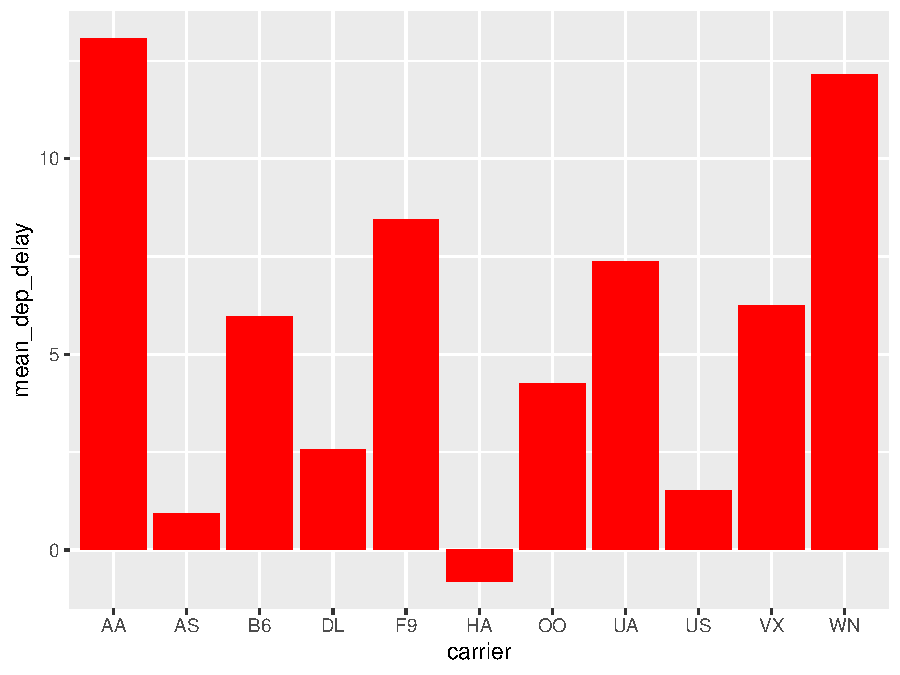
\includegraphics{thesis_files/figure-latex/delaysboxplot-1.pdf}
  \caption{\label{fig:delaysboxplot}Mean Delays by Airline}
  \end{figure}
  Here is a reference to this image: Figure \ref{fig:delaysboxplot}.
  
  A table linking these carrier codes to airline names is available at \url{https://github.com/ismayc/pnwflights14/blob/master/data/airlines.csv}.
  
  \clearpage
  
  Next, we will explore the use of the \texttt{out.extra} chunk option, which can be used to shrink or expand an image loaded from a file by specifying \texttt{"scale=\ "}. Here we use the mathematical graph stored in the ``subdivision.pdf'' file.
  \begin{figure}
  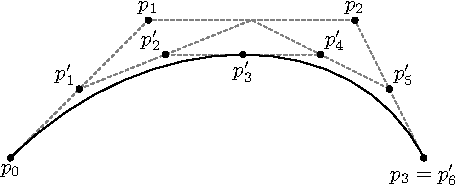
\includegraphics[scale=0.75]{figure/subdivision} \caption{Subdiv. graph}\label{fig:subd}
  \end{figure}
  Here is a reference to this image: Figure \ref{fig:subd}. Note that \texttt{echo=FALSE} is specified so that the \textbf{R} code is hidden in the document.
  
  \textbf{More Figure Stuff}
  
  Lastly, we will explore how to rotate and enlarge figures using the \texttt{out.extra} chunk option. (Currently this only works in the PDF version of the book.)
  \begin{figure}
  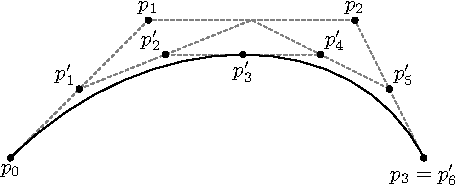
\includegraphics[angle=180, scale=1.1]{figure/subdivision} \caption{A Larger Figure, Flipped Upside Down}\label{fig:subd2}
  \end{figure}
  As another example, here is a reference: Figure \ref{fig:subd2}.
  
  \hypertarget{footnotes-and-endnotes}{%
  \section{Footnotes and Endnotes}\label{footnotes-and-endnotes}}
  
  You might want to footnote something.\footnote{footnote text} The footnote will be in a smaller font and placed appropriately. Endnotes work in much the same way. More information can be found about both on the CUS site or feel free to reach out to \href{mailto:data@reed.edu}{\nolinkurl{data@reed.edu}}.
  
  \hypertarget{bibliographies}{%
  \section{Bibliographies}\label{bibliographies}}
  
  Of course you will need to cite things, and you will probably accumulate an armful of sources. There are a variety of tools available for creating a bibliography database (stored with the .bib extension). In addition to BibTeX suggested below, you may want to consider using the free and easy-to-use tool called Zotero. The Reed librarians have created Zotero documentation at \url{http://libguides.reed.edu/citation/zotero}. In addition, a tutorial is available from Middlebury College at \url{http://sites.middlebury.edu/zoteromiddlebury/}.
  
  \emph{R Markdown} uses \emph{pandoc} (\url{http://pandoc.org/}) to build its bibliographies. One nice caveat of this is that you won't have to do a second compile to load in references as standard LaTeX requires. To cite references in your thesis (after creating your bibliography database), place the reference name inside square brackets and precede it by the ``at'' symbol. For example, here's a reference to a book about worrying: ({\textbf{???}}). This \texttt{Molina1994} entry appears in a file called \texttt{thesis.bib} in the \texttt{bib} folder. This bibliography database file was created by a program called BibTeX. You can call this file something else if you like (look at the YAML header in the main .Rmd file) and, by default, is to placed in the \texttt{bib} folder.
  
  For more information about BibTeX and bibliographies, see our CUS site (\url{http://web.reed.edu/cis/help/latex/index.html})\footnote{({\textbf{???}})}. There are three pages on this topic: \emph{bibtex} (which talks about using BibTeX, at \url{http://web.reed.edu/cis/help/latex/bibtex.html}), \emph{bibtexstyles} (about how to find and use the bibliography style that best suits your needs, at \url{http://web.reed.edu/cis/help/latex/bibtexstyles.html}) and \emph{bibman} (which covers how to make and maintain a bibliography by hand, without BibTeX, at \url{http://web.reed.edu/cis/help/latex/bibman.html}). The last page will not be useful unless you have only a few sources.
  
  If you look at the YAML header at the top of the main .Rmd file you can see that we can specify the style of the bibliography by referencing the appropriate csl file. You can download a variety of different style files at \url{https://www.zotero.org/styles}. Make sure to download the file into the csl folder.
  
  \textbf{Tips for Bibliographies}
  \begin{itemize}
  \tightlist
  \item
    Like with thesis formatting, the sooner you start compiling your bibliography for something as large as thesis, the better. Typing in source after source is mind-numbing enough; do you really want to do it for hours on end in late April? Think of it as procrastination.
  \item
    The cite key (a citation's label) needs to be unique from the other entries.
  \item
    When you have more than one author or editor, you need to separate each author's name by the word ``and'' e.g.~\texttt{Author\ =\ \{Noble,\ Sam\ and\ Youngberg,\ Jessica\},}.
  \item
    Bibliographies made using BibTeX (whether manually or using a manager) accept LaTeX markup, so you can italicize and add symbols as necessary.
  \item
    To force capitalization in an article title or where all lowercase is generally used, bracket the capital letter in curly braces.
  \item
    You can add a Reed Thesis citation\footnote{({\textbf{???}})} option. The best way to do this is to use the phdthesis type of citation, and use the optional ``type'' field to enter ``Reed thesis'' or ``Undergraduate thesis.''
  \end{itemize}
  \hypertarget{anything-else}{%
  \section{Anything else?}\label{anything-else}}
  
  If you'd like to see examples of other things in this template, please contact the Data @ Reed team (email \href{mailto:data@reed.edu}{\nolinkurl{data@reed.edu}}) with your suggestions. We love to see people using \emph{R Markdown} for their theses, and are happy to help.
  
  \hypertarget{conclusion}{%
  \chapter*{Conclusion}\label{conclusion}}
  \addcontentsline{toc}{chapter}{Conclusion}
  
  If we don't want Conclusion to have a chapter number next to it, we can add the \texttt{\{-\}} attribute.
  
  \textbf{More info}
  
  And here's some other random info: the first paragraph after a chapter title or section head \emph{shouldn't be} indented, because indents are to tell the reader that you're starting a new paragraph. Since that's obvious after a chapter or section title, proper typesetting doesn't add an indent there.
  
  \appendix
  
  \hypertarget{the-first-appendix}{%
  \chapter{The First Appendix}\label{the-first-appendix}}
  
  This first appendix includes all of the R chunks of code that were hidden throughout the document (using the \texttt{include\ =\ FALSE} chunk tag) to help with readibility and/or setup.
  
  \textbf{In the main Rmd file}
  \begin{Shaded}
  \begin{Highlighting}[]
  \CommentTok{# This chunk ensures that the coppedown package is}
  \CommentTok{# installed and loaded. This coppedown package includes}
  \CommentTok{# the template files for the thesis.}
  \ControlFlowTok{if}\NormalTok{(}\OperatorTok{!}\KeywordTok{require}\NormalTok{(devtools))}
    \KeywordTok{install.packages}\NormalTok{(}\StringTok{"devtools"}\NormalTok{, }\DataTypeTok{repos =} \StringTok{"http://cran.rstudio.com"}\NormalTok{)}
  \ControlFlowTok{if}\NormalTok{(}\OperatorTok{!}\KeywordTok{require}\NormalTok{(coppedown))}
  \NormalTok{  devtools}\OperatorTok{::}\KeywordTok{install_github}\NormalTok{(}\StringTok{"mralbu/coppedown"}\NormalTok{)}
  \KeywordTok{library}\NormalTok{(coppedown)}
  \end{Highlighting}
  \end{Shaded}
  \textbf{In Chapter \ref{ref-labels}:}
  \begin{Shaded}
  \begin{Highlighting}[]
  \CommentTok{# This chunk ensures that the thesisdown package is}
  \CommentTok{# installed and loaded. This thesisdown package includes}
  \CommentTok{# the template files for the thesis and also two functions}
  \CommentTok{# used for labeling and referencing}
  \ControlFlowTok{if}\NormalTok{(}\OperatorTok{!}\KeywordTok{require}\NormalTok{(devtools))}
    \KeywordTok{install.packages}\NormalTok{(}\StringTok{"devtools"}\NormalTok{, }\DataTypeTok{repos =} \StringTok{"http://cran.rstudio.com"}\NormalTok{)}
  \ControlFlowTok{if}\NormalTok{(}\OperatorTok{!}\KeywordTok{require}\NormalTok{(dplyr))}
      \KeywordTok{install.packages}\NormalTok{(}\StringTok{"dplyr"}\NormalTok{, }\DataTypeTok{repos =} \StringTok{"http://cran.rstudio.com"}\NormalTok{)}
  \ControlFlowTok{if}\NormalTok{(}\OperatorTok{!}\KeywordTok{require}\NormalTok{(ggplot2))}
      \KeywordTok{install.packages}\NormalTok{(}\StringTok{"ggplot2"}\NormalTok{, }\DataTypeTok{repos =} \StringTok{"http://cran.rstudio.com"}\NormalTok{)}
  \ControlFlowTok{if}\NormalTok{(}\OperatorTok{!}\KeywordTok{require}\NormalTok{(ggplot2))}
      \KeywordTok{install.packages}\NormalTok{(}\StringTok{"bookdown"}\NormalTok{, }\DataTypeTok{repos =} \StringTok{"http://cran.rstudio.com"}\NormalTok{)}
  \ControlFlowTok{if}\NormalTok{(}\OperatorTok{!}\KeywordTok{require}\NormalTok{(thesisdown))\{}
    \KeywordTok{library}\NormalTok{(devtools)}
  \NormalTok{  devtools}\OperatorTok{::}\KeywordTok{install_github}\NormalTok{(}\StringTok{"ismayc/thesisdown"}\NormalTok{)}
  \NormalTok{  \}}
  \KeywordTok{library}\NormalTok{(thesisdown)}
  \NormalTok{flights <-}\StringTok{ }\KeywordTok{read.csv}\NormalTok{(}\StringTok{"data/flights.csv"}\NormalTok{)}
  \end{Highlighting}
  \end{Shaded}
  \hypertarget{the-second-appendix-for-fun}{%
  \chapter{The Second Appendix, for Fun}\label{the-second-appendix-for-fun}}
  
  This first appendix includes all of the R chunks of code that were hidden throughout the document (using the \texttt{include\ =\ FALSE} chunk tag) to help with readibility and/or setup.
  
  \backmatter
  
  \hypertarget{referuxeancias-bibliogruxe1ficas}{%
  \chapter*{Referências Bibliográficas}\label{referuxeancias-bibliogruxe1ficas}}
  \addcontentsline{toc}{chapter}{Referências Bibliográficas}
  
  \markboth{References}{References}
  
  \label{bib:begin}
  \noindent
  
  \setlength{\parindent}{-0.20in}
  \setlength{\leftskip}{0.20in}
  \setlength{\parskip}{8pt}
  
  \hypertarget{refs}{}
  \leavevmode\hypertarget{ref-teste-1}{}%
  ABRAHAM, A., MARSDEN, J. E., RATIU, T. \textbf{Aanifolds, Tensor Analysis, and Applications}. Tradução:. 2. ed. New York, Springer-Verlag, 1988.
  
  \leavevmode\hypertarget{ref-book-example}{}%
  ABRAHAM, R., MARSDEN, J. E., RATIU, T. \textbf{Manifolds, Tensor Analysis, and Applications}. Tradução:. 2. ed. New York, Springer-Verlag, 1988.
  
  \leavevmode\hypertarget{ref-teste-2}{}%
  ABRAHAM, Z., MARSDEN, J. E., RATIU, T. \textbf{zanifolds, Tensor Analysis, and Applications}. Tradução:. 2. ed. New York, Springer-Verlag, 1988.
  
  \leavevmode\hypertarget{ref-incollection-example}{}%
  COWIN, S. C., "Adaptive Anisotropy: An Example in Living Bone". In:, \textbf{Non-Classical Continuum Mechanics}, London Mathematical Society Lecture Note Series. Tradução:. {[}S.l.{]}, Cambridge University Press, 1987. v. 122. p. 174--186.
  
  \leavevmode\hypertarget{ref-inbook-example}{}%
  EDWARDS, D. K., "Thermal Radiation Measurements". In: ECKERT, E. R. G., GOLDSTEIN, R. J. (Ed.), \textbf{Measurements in Heat Transfer}, Tradução:. 2. ed. New York, USA, Hemisphere Publishing Corporation, 1976..
  
  \leavevmode\hypertarget{ref-techreport-exampleIn}{}%
  GARRET, D. A. \textbf{The Microscopic Detection of Corrosion in Aluminum Aircraft Structures with Thermal Neutron Beams and Film Imaging Methods}. In: Report, nº NBSIR 78-1434. Washington, D.C., National Bureau of Standards, 1977.
  
  \leavevmode\hypertarget{ref-inproceedings-example}{}%
  GURTIN, M. E. "On the nonlinear theory of elasticity". In:, ago. 1977. \textbf{Anais} {[}\ldots{]} Rio de Janeiro, {[}s.n.{]}, ago. 1977. p. 237--253.
  
  \leavevmode\hypertarget{ref-article-example}{}%
  IESAN, D. "Existence Theorems in the Theory of Mixtures", \textbf{Journal of Elasticity}, v. 42, n. 2, p. 145--163, fev. 1996..
  
  \leavevmode\hypertarget{ref-techreport-example}{}%
  MAESTRELLO, L. \textbf{Two-Point Correlations of Sound Pressure in the Far Field of a Jet: Experiment}. NASA, nº TM~X-72835. {[}S.l: s.n.{]}, 1976.
  
  \leavevmode\hypertarget{ref-phdthesis-example}{}%
  PAES JUNIOR, H. R. \textbf{Influência da Espessura da Camada Intrínseca e Energia do Foton na Degradação de Células Solares de Silício Amorfo Hidrogenado}. 1994. Tese de D.Sc. -- COPPE/UFRJ, Rio de Janeiro, RJ, Brasil, 1994.
  
  \leavevmode\hypertarget{ref-mastersthesis-example}{}%
  TUNTOMO, A. \textbf{Transport Phenomena in a Small Particle with Internal Radiant Absorption}. 1990. Ph.D. dissertation -- University of California at Berkeley, Berkeley, California, USA, 1990.

  \backmatter
  \bibliographystyle{coppe-unsrt}
  \bibliography{thesis}

  %\appendix
  %\include{appenA}
\end{document}
